\documentclass{article}
\usepackage{fixltx2e}
\usepackage{float}
\usepackage{amsmath}
\newcommand{\degree}{\ensuremath{^\circ}}
\usepackage{graphicx}
\usepackage[margin=1.0in]{geometry}
\linespread{1.5}


\title{Progress Report: An Agent Based Financial Market}

\author{Michael Lee \\*
The University of Texas at Austin}

\begin{document}

\maketitle{}


The goal of the final project is to combine the agent based modeling techniques used to model resource allocation and portfolio optimization to create a fully functioning financial market. Agents will be randomly assigned existing portfolio parameters including risk-aversion and duration, while new parameters from the agent based model will be integrated into the optimization criteria, including wealth and quantity demanded. Based on the agent's optimization criteria, they purchase stock; their demand drives up the call price for the next agent. This process is repeated-- at each turn the agents get can buy our sell their portfolio to maximize utility based on the adjusted prices. The resulting feedback loop is meant to model a financial market, where the prices are dynamic and related to the number of agents purchasing and selling at each turn. 

\newpage{}

\section{Portfolio Optimization}
The portfolio optimization algorithm used in previous papers form the basis of this model, however some adjustments are be made. As in the original model: historical data is used to predict future prices; the volatility of the entire portfolio is calculated using matrix operations to show the virtuous effects of diversification as suggested by Markowitz in his 1952 paper on Modern Portfolio Theory (Markowitz, 1990); a more modern method of calculating asset volatility is built-in such that recent volatility is more heavily weighted. 

\subsection{Accounting}
In the previous model, the buyer was assumed to have all the money necessary to purchase any of the listed assets. Also, agents were allowed to purchase fractional assets, something that could not happen in real life (excluding mutual funds). This model was an oversimplification and led to the optimal portfolios having large portions of Apple and Google stock, the two most expensive. \*

In the new model, each agent is randomly assigned some measure of wealth, which limits the assets he or she can buy. This measure of wealth will be the inequality constraint in the optimization problem. Initially all wealth is in the form of cash, but after the fist turn the wealth is the combined sum of the assets held and remaining cash. At each turn, the agent has the option to liquidate assets at the current price and purchase a new portfolio.

\subsection{Optimization}
For this model there is a fundamental differences in how the optimization problem is formulated. Instead of using Monte-Carlo simulations to randomly generate the distribution of assets held, an analytical expression is created. This formula is a quintessential constrained optimization problem: maximize expected utility subject to a price constraint. 


\begin{equation}
	 max:EU(\pi, EWMA, \beta, \delta\ t) = 1 - exp(-\beta \frac{\pi}{EWMA}\delta^t)
\end{equation}

\begin{equation}
	s.t.: \Sigma{P_{assets} * N_{assets}} < Wealth_{agent}
\end{equation}

This is a significantly more complex optimization problem than the previous Monte-Carlo method, but allows for the wealth of the individual agent to be factored in, as well as being more computationally efficient than randomly generating 500 portfolios for multiple agents. 

\subsection{Dynamic Pricing}
The final step of making the financial market is to create a dynamic pricing mechanism. Dynamic pricing implies that at each turn, the number of shares being sold and bought will affect the price of the asset. \emph{this has also proved to be more difficult than originally imagined}. As of now, I cannot find a mechanism that will effectively price assets based off a) their original price, b) the normalized number of outstanding shares, and c) the number of agents buying and selling at each turn. The implementation of dynamic pricing however, is at this time the cornerstone of an agent based model, as it requires each agent consider the actions of other agents. For this reason, it cannot be omitted.


\section{Agent Based Markets}
The market is fully created when multiple agents, each with their own optimization problem, are set into a market where the price of their assets are changing depending on the optimization problems of their neighbors. In this regard, the model accurately represents the problems faced by investors in the real world. 

\subsection{Agent Characteristics}
In order to simulate the diversity of retail investors, each agent is randomly assigned some initial wealth, a level of risk-aversion, and a duration or time in which they want to liquidate all their assets and leave the market. These factors are given in the initialization of the program, and with the exception of wealth, remain static throughout. \*

The level of wealth however, changes at each turn as the value of the assets held fluctuates. Thus, some agents will become richer or poorer based on the amount of demand for the assets they hold. This will cause them to sell off their portfolio, and depending on their risk aversion, purchase a different set of assets. \*

If time permits, I would also like to incorporate a changing risk-aversion over time, where as the agents get older (more turns pass), they become more and more risk-adverse as they prepare to leave the market (retire). 

\subsection{Purchasing}
After initialization, agents are randomly permutated for the order in which they get to enter the market. Each agent then choses to purchase the assets that optimize their portfolio following {\bf Equations 1, 2}. After each agent, the prices are updated to reflect the amount of each asset purchased. This will cause the first few agents to have the best chance at maximizing utility-- a phenomenon seen in the real world in early investors. A functional diagram of the market is seen below.   

\begin{figure}[H]
	\begin{center}
		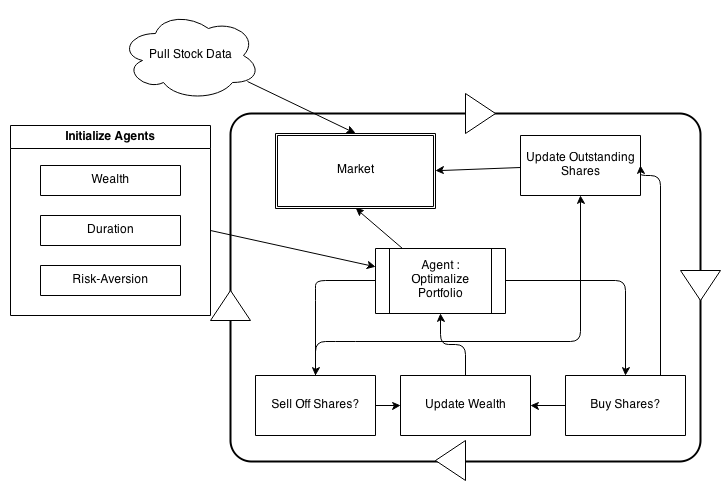
\includegraphics[scale= .7]{market_flowchart.png}
		\caption{Flowchart of the Dynamic Market}
	\end{center}
\end{figure}

\section{Moving Forward}
Much of the project is already in place, however the mechanism for updating prices still needs to be created. This will prove difficult, but I believe that (maybe with some help!) it can be modeled computationally. In addition, this dynamic game will most likely need to be run on a computer more powerful than my little laptop, so I will try and port it to run on the HPC node made available by the mechanical engineering department. I hope to be able to make this computationally elegant, and maybe incorporate some of the techniques I've learned in my Computational ThermoFluid Systems class, such as the development of stable algorithms and the use of Largrangians to transform constrained optimization problems to simpler, unconstrained optimization problems. 





\end{document}
